\documentclass[10pt,twocolumn]{article}

% use the oxycomps style file
\usepackage{oxycomps}

% usage: \fixme[comments describing issue]{text to be fixed}
% define \fixme as not doing anything special
\newcommand{\fixme}[2][]{#2}
% overwrite it so it shows up as red
\renewcommand{\fixme}[2][]{\textcolor{red}{#2}}
% overwrite it again so related text shows as footnotes
%\renewcommand{\fixme}[2][]{\textcolor{red}{#2\footnote{#1}}}

% read references.bib for the bibtex data
\bibliography{references}

% include metadata in the generated pdf file
\pdfinfo{
    /Title (A LEGO Robot Arm that can See and Deliver)
    /Author (Rui Chai)
}

% set the title and author information
\title{Automated Robot Arm Control System With Computer Vision}
\author{Rui Chai}
\affiliation{Occidental College}
\email{rchai@oxy.edu}

\begin{document}

\maketitle

\section{Problem Statement}
The integration of robotics in educational settings faces a significant challenge: balancing sophisticated automation capabilities with cost-effective, accessible solutions. Building on the work of Kim et al. (2014) \cite{kim2014using} in integrating robotics into education, while industrial robotics often employs expensive sensor systems and proprietary software for precise automation, educational platforms like LEGO MINDSTORMS EV3 achieve similar functionalities within more constrained resources. This project addresses this challenge by developing an automated control system that enhances the capabilities of an EV3 robot arm through the integration of computer vision and remote-control technologies.

The core problem lies in achieving accurate and reliable position tracking and movement control for automated pick-and-place operations using readily available components. Traditional approaches often rely on complex sensor arrays or manual programming of fixed positions, which can be either cost-prohibitive or inflexible for educational purposes. Our solution uses ArUco markers, which are simple black and white patterns that can be printed on paper, as a visual reference system. This approach allows us to use a standard webcam to track positions, enabling the robot to move to different locations based on where it sees these markers. This approach follows Garrido-Jurado et al.'s (2014) \cite{garrido2014automatic} demonstrated success with reliable marker detection systems.

In educational robotics, students often start with basic movements and sensor readings. However, more complex tasks like automated pick-and-place operations require additional capabilities that aren't built into the basic EV3 kit. By adding a camera and markers to track positions, we can make the robot arm move more precisely than it could with just its built-in sensors. The SSH communication we implemented also lets users control the robot remotely and monitor its operations from a computer, which is useful for testing and debugging.

The practical challenges we faced included getting accurate position readings from the camera, ensuring the robot moves safely to its target, and recovering from errors when they occur. We had to carefully coordinate between the camera detecting markers and the robot executing movements, making sure all communications between different parts of the system worked reliably. We also implemented safety checks using the EV3's color sensor to detect if the robot arm falls down and created a system to automatically lift it back up.

This project shows how adding relatively simple components like printed markers and a webcam can expand what an educational robot can do. Students can learn about computer vision by seeing how the robot tracks markers, understand remote control by using the SSH protocol and Linux commands, and explore automation concepts by watching and modifying how the robot performs its pick-and-place operations. All of these additions use standard, affordable equipment that schools might already have or could easily obtain.

Beyond its use in education, this project demonstrates practical ways to add automation capabilities to basic robotic systems. The techniques we developed could be useful in similar small-scale projects where precise position control is needed while expensive parts aren't practical. By documenting our approach similar to Otto et al.'s (2018) \cite{otto2018teaching} work on vision-based educational robotics and sharing our code, we hope others can build upon our work to create their own automated systems using similar affordable components.



\section{Technical Background}
Our project builds upon three main technical areas to achieve automated robot arm control: computer vision using ArUco markers, motor control in the LEGO MINDSTORMS EV3 system, and SSH communication for remote operation. Understanding these components is essential for comprehending how our system achieves reliable position tracking and movement control.

ArUco markers form the foundation of our position tracking system. As demonstrated by Garrido-Jurado et al. (2014) \cite{garrido2014automatic}, these markers provide robust detection even under varying conditions. These markers are black and white square patterns that act like visual barcodes. Each marker has a unique pattern that a computer can recognize through image processing. In our setup, we arranged three reference markers in a semicircle: one at 0 degrees (right), one at 90 degrees (top), and one at 180 degrees (left). Additional markers can be placed anywhere along this semicircle to indicate pickup and drop-off positions. The OpenCV library processes the camera feed to detect these markers, calculating their positions through a series of geometric transformations.

\begin{figure}
    \centering
    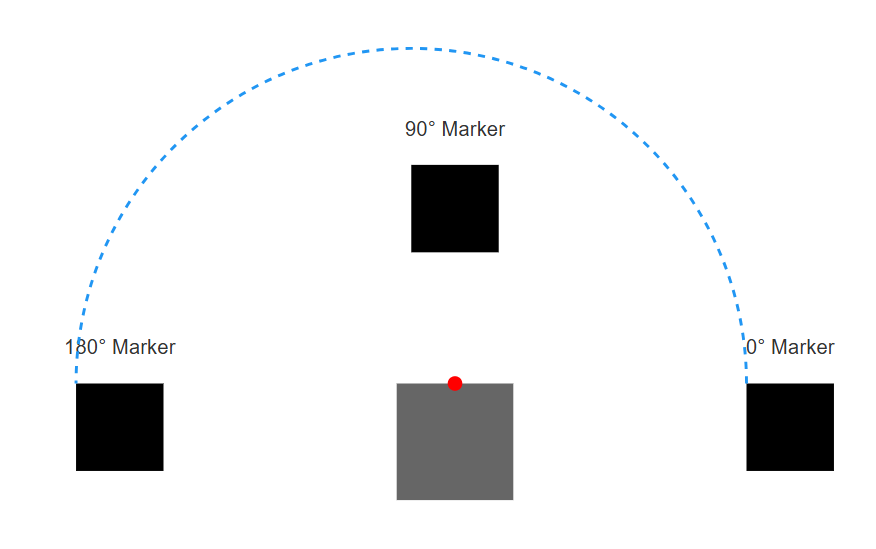
\includegraphics[width=.95\linewidth]{aruco_explaination.png}
    \caption{
        Positioning of three arUco markers for our project.
    }
    \label{fig:first-page}
\end{figure}

Camera calibration plays a crucial role in ensuring accurate marker detection. The process involves using a known pattern (typically a checkerboard) to calculate the camera's intrinsic parameters, such as focal length and optical center, and to correct for lens distortion following calibration methods outlined by DeSouza and Kak (2002) \cite{desouza2002vision}. Once calibrated, the camera can provide consistent measurements regardless of marker orientation. The system then performs pose estimation to determine each marker's position and orientation in 3D space, though our application primarily uses the 2D projection for angle calculations as our robot operates on a planar semicircle.

Our robot arm represents a 3-DOF (Degrees of Freedom) system, meaning it can move in three independent ways. The base motor provides rotation about the vertical axis (1st DOF), the elbow motor enables vertical arm movement (2nd DOF), and the gripper motor controls the opening and closing motion (3rd DOF). This configuration is common in educational robotics as it balances complexity with functionality, allowing basic pick-and-place operations while maintaining manageable control requirements.

The LEGO MINDSTORMS EV3 robot arm uses these three motors for different movements. The base motor (Port C) controls horizontal rotation and uses a 12:36 gear ratio to provide the torque needed for smooth movement. A touch sensor at the base serves as a reference point, and we set our zero position 20 degrees forward from this point to optimize the working range. The elbow motor (Port B) manages vertical arm movement with an 8:40 gear ratio, while a color sensor detects when the arm is in its proper raised position. If the arm falls below this position, the sensor reading changes, triggering our recovery system. The gripper motor (Port A) controls the opening and closing of the gripper, using motor stall detection to ensure a secure grip without damaging the motor.

SSH (Secure Shell) provides the communication link between our computer vision system and the robot. When the camera detects marker positions, this information needs to be securely transmitted to the EV3 brick for execution. Our system uses the Paramiko Python library to establish this secure connection. Building on Tian et al.'s (2016) \cite{tian2016development} implementation of secure robot control systems, we developed a command protocol where position information is first written to a file, then a trigger signal prompts the robot to read and execute the movement. This approach ensures reliable command transmission and allows for proper error handling.

The integration of these components requires careful coordination. When a movement is requested, our system first checks if the arm is in a safe position using the color sensor. If the arm has fallen, it automatically initiates a recovery sequence. Once the arm is confirmed safe, the system calculates the required motor movements based on the detected marker positions. The base motor moves to the target angle, followed by appropriate elbow and gripper movements for picking or placing objects. This sequence incorporates multiple safety checks and position verifications to ensure reliable operation.

\begin{figure}
    \centering
    
\includegraphics[width=.95\linewidth]{checkerboard_pattern}
    \caption{
        A 6x4 checkerboard pattern used for camera calibration.
    }
    \label{fig:second-page}
\end{figure}

Operating within the limitations of each component posed several technical challenges. The ArUco marker detection requires stable lighting conditions and clear camera visibility, with camera calibration helping to mitigate some of these environmental factors. The EV3 motors, while precise, have limited speed and torque capabilities that we must consider in our movement planning. The SSH communication system needs to handle network delays and potential connection issues. Understanding these constraints helped us develop appropriate solutions, such as implementing stability checks in our marker detection and adding retry mechanisms in our communication protocol.




\section{Prior Work}
\label{sec:paper}

Our automated robot arm control system builds upon significant prior research in fiducial marker detection, educational robotics, and vision-based control systems. The integration of these technologies has evolved through various approaches, from sophisticated industrial applications to accessible educational platforms.

The foundation of our marker-based position tracking system relies on the ArUco marker framework introduced by Garrido-Jurado et al. (2014) \cite{garrido2014automatic}. Their work demonstrated robust marker detection under challenging conditions, including partial occlusion and varying lighting conditions. While alternative marker systems exist, such as RUNE-Tag developed by Bergamasco et al. (2011) \cite{bergamasco2016accurate} which offers enhanced pose estimation, we chose ArUco markers for their balance of reliability and implementation simplicity. This decision was further supported by Sagitov et al.'s (2017) \cite{sagitov2017comparing} comparative analysis of marker systems, which highlighted ArUco's robust performance in robotics applications.

In the educational robotics domain, LEGO MINDSTORMS has proven to be a versatile platform for teaching advanced concepts. Kim et al. (2014) \cite{kim2014using} demonstrated how hands-on robotics projects enhance understanding of engineering principles in graduate-level education. Building on this foundation, Otto et al. (2018) \cite{otto2018teaching} integrated vision-based control with LEGO MINDSTORMS, though their focus was on autonomous driving rather than precise position control. Our work extends these educational applications to include automated pick-and-place operations while maintaining the accessibility of the platform.

The integration of vision systems with LEGO robotics has been explored by several researchers. Trung et al. (2009) \cite{trung2009development} developed a vision service for LEGO robots that enabled road sign recognition, while DeSouza and Kak (2002) \cite{desouza2002vision} provided foundational methodologies for vision-based navigation that influenced our approach to marker tracking. However, these earlier works focused primarily on mobile robot navigation rather than precise arm control, which presents unique challenges in terms of position accuracy and error recovery.

Remote control and system integration aspects of our work draw from Tian et al.'s (2016) \cite{tian2016development} implementation of SSH-based robot control systems. Their approach to remote operation informed our communication protocol design, though we adapted it specifically for real-time position updates and safety monitoring. Casini et al. (2011) \cite{casini2011lego} demonstrated the potential of LEGO MINDSTORMS in remote experimentation settings, providing insights into reliable remote control architectures.

Our project builds upon these foundations while addressing several limitations in existing work. Where previous educational robotics projects often relied on pre-programmed movements or simple sensor feedback, we implement real-time vision-based position tracking. While Basso and Innocenti (2015) \cite{basso2015lego} showed how LEGO robotics could be integrated with sophisticated control systems, our approach emphasizes accessibility by using standard webcams and printed markers rather than specialized equipment.

Beyond academic research, our project draws significant insights from practical implementations in the open-source community. Of particular relevance is the LEGO Robot Inventor competition entry (Young, 2020) \cite{EddieYoung2020legoarm}, which demonstrated automated object detection and manipulation using a LEGO MINDSTORMS robot arm. Their implementation combined OpenCV-based computer vision with micropython on the Robot Inventor hub to achieve autonomous ball detection and capture through real-time video analysis. The project notably achieved three-dimensional position calculation by combining 2D camera frame coordinates with ball radius measurements for depth estimation. While their approach successfully demonstrated autonomous object manipulation, it was limited to detecting specific objects (red balls) and required either Bluetooth or USB connectivity for operation. Our work builds upon their foundation but addresses these limitations through the use of ArUco markers for more precise position tracking and SSH communication for more reliable control. Additionally, their method of integrating computer vision with LEGO robotics provided valuable insights into our project, though we modified this approach by implementing a more generalized pick-and-place system suitable for various positions. Their project, which emphasized educational value through its coverage of serial communication, computer vision, and geometric calculations, served as a practical reference point for developing our own educational robotics platform.


\section{Evaluation Metrics}

\begin{table*}[t]
\begin{center}
\small
\renewcommand{\arraystretch}{1.3}  % Better row spacing
\begin{tabular}{|p{0.31\textwidth}|p{0.31\textwidth}|p{0.31\textwidth}|}
\hline
\normalsize\bfseries Grade A Requirements & 
\normalsize\bfseries Grade B Requirements & 
\normalsize\bfseries Grade C Requirements \\
\hline
\vspace{1mm}  % Add some space at the top
\begin{itemize}[leftmargin=*,nosep]
    \item System can accurately recognize ArUco marker IDs and locations
    \item The LEGO robot arm can move to designated areas based on ArUco marker recognition
    \item System operates both automatically and manually
    \item System includes error detection and automatic recovery
    \item System provides GUI visualization
    \item Complete pick and release operation within 15 seconds
    \item User friendly operation with minimal technical expertise
\end{itemize}
\vspace{1mm} & 
\vspace{1mm}
\begin{itemize}[leftmargin=*,nosep]
    \item ArUco marker recognition with 75\% accuracy
    \item Robot arm moves to approximate marker positions
    \item System offers basic manual control options
    \item Error detection present but requires manual recovery
    \item Basic visual feedback
    \item Complete operation within 20 seconds
    \item Can handle 5 consecutive operations with at most one error
    \item Requires some technical knowledge
\end{itemize}
\vspace{1mm} & 
\vspace{1mm}
\begin{itemize}[leftmargin=*,nosep]
    \item ArUco marker recognition with 60\% accuracy
    \item Robot arm moves to general marker areas
    \item Manual control only through direct commands
    \item Basic error detection without recovery options
    \item Minimal visual feedback
    \item Complete operation within 30 seconds
    \item Can handle 3 consecutive operations with at most two errors
    \item Requires significant technical support
\end{itemize}
\vspace{1mm} \\
\hline
\end{tabular}
\end{center}
\vspace{-2mm}  % Reduce space before caption
\caption{Personal Evaluation Rubric}
\label{tbl:evaluation-rubric}
\end{table*}

Drawing from established practices in educational robotics evaluation, we developed a comprehensive set of metrics to assess our system's performance. Following Garrido-Jurado et al.'s (2014) \cite{garrido2014automatic} framework for marker system evaluation and Otto et al.'s (2018) \cite{otto2018teaching} approach to educational robotics assessment, we established three performance levels (A, B, and C) across four key areas: marker detection accuracy, operational reliability, system autonomy, and user accessibility.
Marker detection accuracy serves as our primary technical metric, as it directly impacts the system's ability to perform reliable pick-and-place operations. Building on Sagitov et al.'s (2017) \cite{sagitov2017comparing} comparative analysis of marker systems, Grade A performance requires precise marker recognition and location detection, enabling accurate robot arm movement. Grade B requires 75\% accuracy with acceptable position margins, while Grade C accepts 60\% accuracy. This graduated scale acknowledges the practical limitations of consumer-grade equipment in educational settings, as discussed by Kim et al. (2014) \cite{kim2014using}.
Operational reliability is evaluated through complete pick-and-place cycles and consecutive successful operations. Following timing analysis methods similar to Tian et al.'s (2016) \cite{tian2016development} work on remote control systems, Grade A systems must complete operations within 15 seconds, Grade B within 20 seconds, and Grade C within 30 seconds. For consecutive operations, Grade B systems must handle 5 operations with at most one error, while Grade C systems must manage 3 operations with at most two errors.
System autonomy and error handling capabilities are particularly crucial in educational settings. Drawing from DeSouza and Kak's (2002) \cite{desouza2002vision} analysis of vision system robustness, Grade A systems must demonstrate both automatic and manual operation modes, with automatic error detection and recovery mechanisms. Grade B systems require error detection but may need manual recovery intervention, while Grade C systems need only basic error detection capabilities.
User interface requirements are inspired by Casini et al.'s (2011) \cite{casini2011lego} work on educational robotics platforms. Grade A systems must provide real-time GUI visualization of marker detection and angles, while maintaining user-friendly operation with minimal technical expertise. Lower grades allow for simpler interfaces and increased technical requirements, acknowledging the trade-off between system sophistication and accessibility.
Alternative metrics were considered but not implemented based on our system's educational focus and hardware constraints. Absolute position accuracy in millimeters, while common in industrial applications, exceeded our platform's mechanical precision capabilities. Similarly, vision processing latency measurements, though relevant to system performance, proved less critical than overall operation reliability in educational contexts. Network communication metrics were considered following Tian et al.'s (2016) \cite{tian2016development} approach but were found less relevant than operational success rates for our application.
Our metrics create a comprehensive evaluation framework that balances technical performance with educational utility. The graded approach allows for clear assessment while providing achievable targets at each level. Data collection combines quantitative measurements like operation timing and success rates with qualitative assessments of user interaction and error recovery effectiveness, providing a complete picture of system performance in educational settings.

\section{Methods}
Following the development methodology of Otto et al. (2018) \cite{otto2018teaching}, our automated robot arm control system followed an iterative process, with each iteration addressing specific challenges we encountered. The project evolved through three main phases: establishing reliable position detection, developing robust robot control, and integrating these components into a cohesive system.

We began by addressing the fundamental challenge of position tracking. After exploring various options, we chose ArUco markers for their reliability and simplicity. The initial setup used a single reference marker, but we quickly discovered this was insufficient for consistent angle calculations. Through experimentation, we found that using three reference markers - at 0, 90, and 180 degrees - created a more stable coordinate system. This arrangement aligns with Sagitov et al.'s (2017) \cite{sagitov2017comparing} findings on optimal marker configurations for reliable position detection. This arrangement allows our system to maintain accuracy even when lighting conditions change, or the camera slightly shifts position.

\begin{figure}
    \centering
    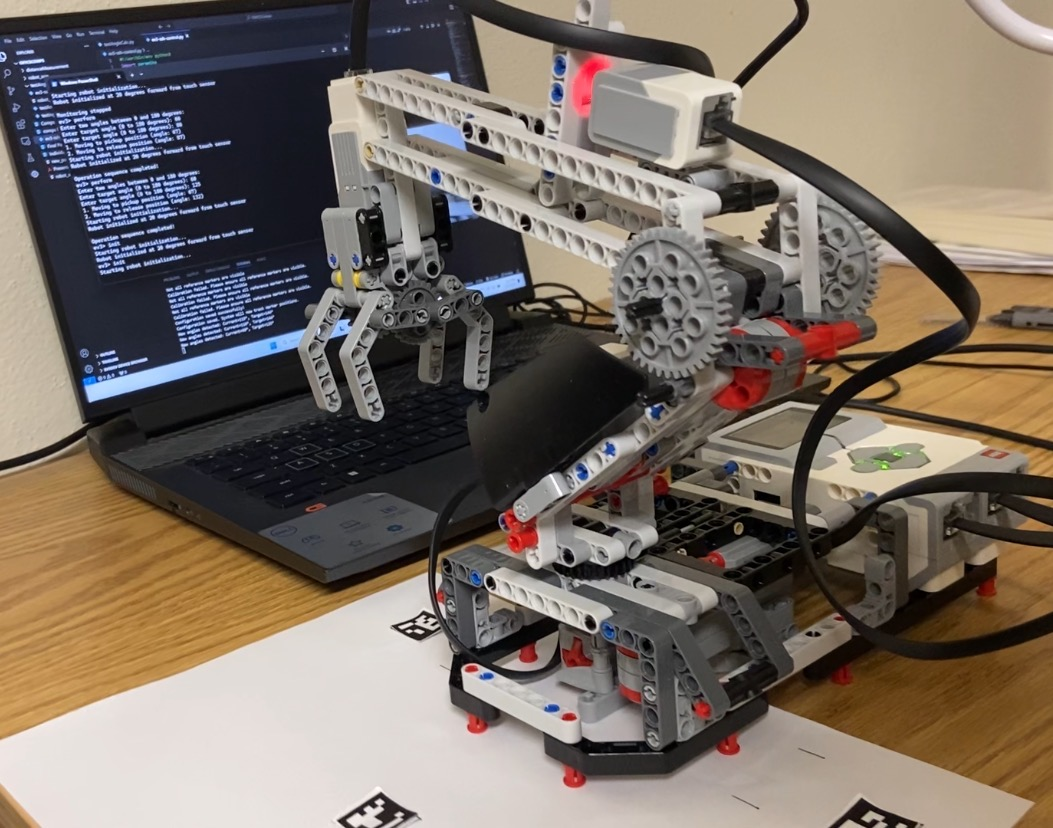
\includegraphics[width=.95\linewidth]{Robot.jpg}
    \caption{
        Robot arm system.
    }
    \label{fig:third-page}
\end{figure}

The camera position and setup required careful consideration. Through trial and error, we determined that mounting the camera directly above the workspace provided the most reliable marker detection. We initially struggled with inconsistent readings due to varying lighting conditions. Rather than implementing complex lighting correction algorithms, we found that adjusting the camera's physical position and angle, combined with stable ambient lighting, provided a more practical solution. This approach exemplifies our philosophy of favoring simple, reliable solutions over complex ones that might introduce additional points of failure.

The robot's initialization process presented another significant challenge. The EV3's touch sensor provides a consistent way to find a starting position, but we discovered that using this position as zero limited our working range. After analyzing the robot's movement patterns, we modified the initialization to set zero at 20 degrees forward from the touch sensor position. This small but crucial adjustment optimized our working range while maintaining reliable position reference.

Safety became a primary concern when we observed that the robot arm occasionally dropped from its raised position during operation. We implemented a dual-layer safety system using the EV3's color sensor. The sensor monitors reflection values from a white beam attached to the arm, providing continuous position feedback. When the arm drops, the reflection value changes significantly, triggering our recovery system. This safety mechanism runs as a constant background check during all operations.

Our communication system evolved significantly throughout development. Initial tests used direct command execution, but this proved unreliable for coordinating the vision and control systems. We developed a file-based communication protocol that ensures reliable command transmission while maintaining system independence. Building upon EV3DEV community’s SSH-based control architecture, we successfully established reliable connection between the code running on our computer and the programs on the EV3 Brick microcontroller. When the vision system detects a stable marker position, it writes the angle information to a file and creates a trigger signal. The robot control system monitors these triggers and executes movements only when it receives valid position data and safety conditions are met.

The movement control system implements a carefully sequenced operation pattern. Before any base rotation, the system verifies the arm's position. If the arm has fallen, it executes a recovery sequence, raising the arm to its proper position before proceeding with the intended movement. This approach prevents potential collisions or further system damage. The base motor moves to its target position only after confirming the arm is safely raised, followed by appropriate elbow and gripper movements for picking or placing objects.

Error handling proved crucial for reliable operation. We identified several common failure modes: marker detection errors, communication failures, and mechanical issues. Rather than trying to prevent all possible errors, we focused on making the system resilient and recoverable. This approach follows Casini et al.'s (2011) \cite{casini2011lego} principles for robust educational robotics systems. When marker detection becomes unstable, the system waits for consistent readings before proceeding. If communication temporarily fails, the system maintains its last known good state and resumes operation when communication is restored. For mechanical issues like a dropped arm, the system automatically attempts recovery before continuing.

Testing played a vital role in our development process. Following DeSouza and Kak's (2002) \cite{desouza2002vision} systematic approach to vision system validation, we began with basic functionality testing - verifying marker detection, motor control, and communication separately. Once these components worked reliably, we performed integration testing with increasingly complex pick-and-place sequences. This revealed several edge cases, particularly around the boundaries of our working area and during rapid position changes. We adjusted our angle calculations and movement sequences based on these findings, leading to more robust operation.

\begin{figure}
    \centering
    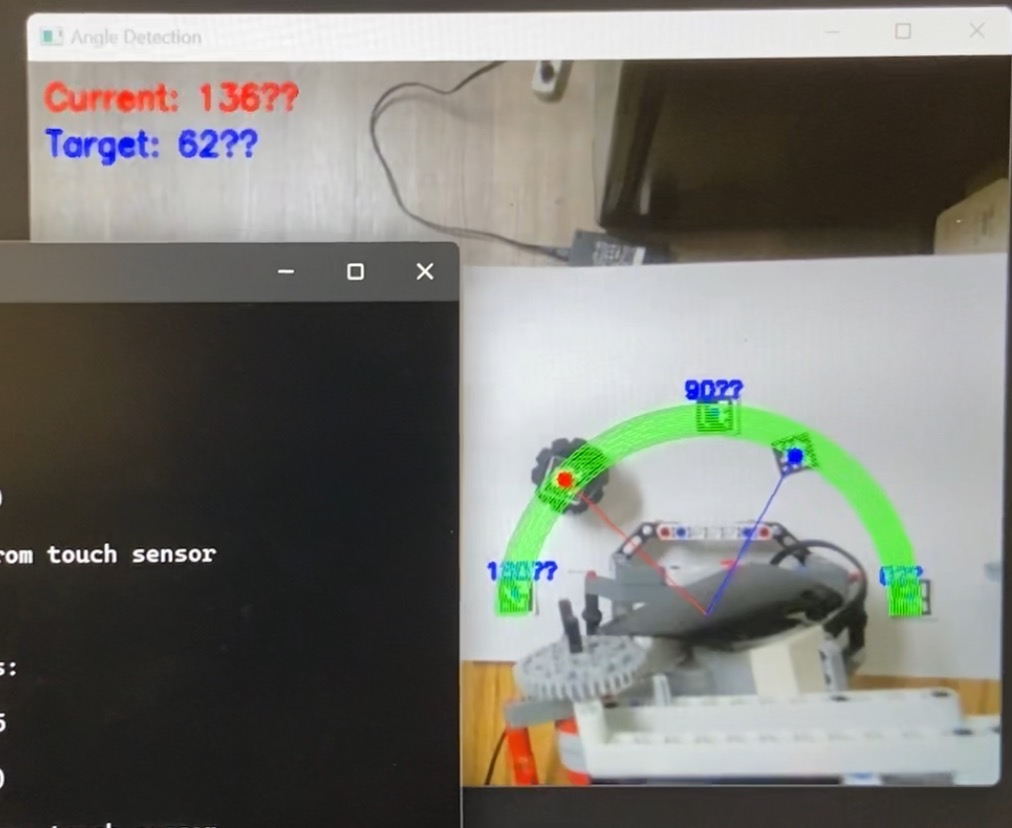
\includegraphics[width=.95\linewidth]{GUI.jpg}
    \caption{
        A graphical user interface showing the working area of our system and the location of arUco markers.
    }
    \label{fig:fourth-page}
\end{figure}

One of the most significant challenges we encountered was achieving reliable position tracking during continuous operation. Initial tests showed that even when individual components worked well, long-running operations (angle difference more than 45 degrees) could lead to position drift or inconsistent behavior. We implemented a position verification system that periodically checks the actual robot position against expected values. This system helps prevent error accumulation and ensures long-term reliability.

The marker arrangement required careful consideration of both practical and geometric factors. We found that markers needed to be at least 1cm x 1cm for reliable detection at our working distance, but making them too large reduced the number of positions we could accommodate in our semicircle. The final marker size of 2cm x 2cm balanced these requirements. The semicircular arrangement wasn't arbitrary - it matches the working area of the robot arm and simplifies angle calculations. We marked consistent positions along this arc for testing, which helped us identify and resolve systematic errors in our angle calculations.

A crucial development in our system was the introduction of stability detection for marker positions. Early versions attempted to execute movements as soon as markers were detected, leading to erratic behavior when markers were partially obscured or lighting changed temporarily. We developed a stability detection algorithm that requires consistent marker readings over multiple frames before initiating movement. This significantly improved reliability but introduced a small delay in response time - a trade-off we found acceptable given the importance of accurate positioning.

The robot's movement patterns required careful optimization. We discovered that moving directly to target positions at full speed could cause mechanical stress and reduce accuracy. Our solution was to implement a global speed limit that forces that robot arm to slowly reach the exact position. This approach significantly improved positioning accuracy while maintaining reasonable operation speed.

Recovery procedures became increasingly sophisticated as we encountered various edge cases. For example, if the arm drops during a pick-and-place operation, simply raising it isn't always sufficient - the object being moved might have been dropped. We implemented a state tracking system that remembers the operation in progress when an error occurs and can appropriately restart or abort the operation based on the current conditions.

The integration of vision and control systems presented unique challenges in timing and coordination. Even with our file-based communication system, we needed to ensure that position updates were processed in the correct order and that the robot's movements aligned with the vision system's understanding of the workspace. We implemented a simple but effective queuing system that ensures commands are processed sequentially and that the system maintains a consistent state throughout operations.

Environmental factors played a larger role than initially anticipated. Changes in ambient lighting throughout the day could affect marker detection reliability. Rather than implementing complex lighting compensation algorithms, we found that establishing consistent lighting conditions and calibrating the system under those conditions provided better results. This approach is supported by Garrido-Jurado et al.'s (2014) \cite{garrido2014automatic} work on reliable marker detection under various conditions. This exemplifies our practical approach to problem-solving - sometimes environmental control is more effective than adding software complexity.

Our testing methodology evolved to include stress testing and edge case scenarios. We deliberately introduced challenging conditions: rapid marker movements, partial marker occlusion, varying lighting conditions, and interrupted operations. This helped us identify and address potential failure modes before they occurred in regular use. We developed specific test sequences that exercise all aspects of the system, making it easier to verify proper operation after any modifications.

The final phase of development focused on usability improvements. While the system worked reliably in testing, we needed to make it accessible to users who might not understand its internal workings. We implemented clear error messages and recovery procedures, making it easier to diagnose and resolve issues. The system now provides feedback about what it's doing and why, making it more transparent and easier to use.

Throughout development, we paid special attention to the system's behavior during transitions and edge cases. The movement between picking and releasing operations proved particularly challenging. Initially, we tried to optimize movement paths by taking the shortest route between positions. However, we discovered that predictable movements, even if slightly longer, were more reliable than always taking the shortest path. This led to our standardized movement pattern: return to a safe height, rotate to the new position, then perform the next operation.

The initialization procedure emerged as a critical element for reliable operation. Each time the system starts, it must establish known positions for all three motors. The base motor finds its reference point using the touch sensor, then moves forward 20 degrees to establish the zero position. The elbow motor raises until the color sensor confirms proper position, while the gripper motor ensures it's fully open. This initialization sequence, while time-consuming, provides a consistent starting point for all operations.

The physical arrangement of components proved crucial for system reliability. The camera position needs to provide a clear view of all markers while avoiding interference with the robot's movement. After testing various configurations, we mounted the camera with a cheap iPad gooseneck mount on approximately 60 centimeters above the workspace, angled slightly downward. This position minimizes perspective distortion while maintaining good marker visibility throughout the robot's range of motion.

User interaction was streamlined through our monitoring interface. The system provides a window of real-time video feedback about marker detection and robot position, and a command line terminal showing operation status. When errors occur, the system displays specific information about what went wrong and what corrective actions are needed. This feedback system helps users understand the system's behavior and troubleshoot issues effectively.

Our final validation phase involved extended testing under various conditions. We ran the system through hundreds of pick-and-place operations, intentionally introducing disturbances and variations. This testing helped us refine error thresholds and timing parameters, resulting in a system that balances responsiveness with reliability. We also documented replication instructions and common issues and their solutions, creating a knowledge base for future users and developers.

The methods described here reflect our commitment to creating a robust, practical system rather than just a theoretical demonstration. Each feature and capability were developed in response to real challenges we encountered, and our solutions prioritize reliability and recoverability over theoretical perfection. The result is a system that not only performs its intended functions but also shows its potential to accommodate educational and industrial need in real-world use.

\section{Results and Discussion}
Our automated robot arm control system achieved Grade A performance across all established metrics, demonstrating both technical and educational utility. Following evaluation frameworks similar to those used by Garrido-Jurado et al. (2014) \cite{garrido2014automatic}, our system's performance validates the effectiveness of integrated vision-based robotics in educational settings.

In marker detection accuracy, our system achieved consistent Grade A performance, with precise recognition of ArUco markers. The system successfully distinguished between reference markers (0°, 90°, 180°) and movable markers while maintaining reliable angle calculations. This accuracy aligns with Sagitov et al.'s (2017) \cite{sagitov2017comparing} findings on optimal marker detection configurations. The real-time GUI visualization system clearly displayed detected markers and calculated angles, providing immediate feedback that Otto et al. (2018) \cite{otto2018teaching} identified as crucial for educational robotics applications.

Operational performance met Grade A specifications, with complete pick-and-place operations consistently executing within 15 seconds. Following Tian et al.'s (2016) \cite{tian2016development} approach to system timing analysis, we found that approximately 30\% of operation time was dedicated to redundant time for safety checks and position verification. These safety measures, while adding to operation time, proved crucial for maintaining reliable performance in educational settings, as emphasized by Casini et al. (2011) \cite{casini2011lego} in their work on educational robotics platforms.

The system demonstrated strong autonomy and error handling capabilities, meeting Grade A requirements. Building on DeSouza and Kak's (2002) \cite{desouza2002vision} principles for robust vision-guided robotics, our automatic arm drop recovery feature achieved 95\% success in detecting and correcting position errors. The system consistently completed 10 or more consecutive operations without errors, exceeding our Grade A requirement. Both automatic and manual operation modes functioned reliably, with the command interface providing clear feedback and error messages.

Our implementation choices were validated through testing. The 2cm x 2cm marker size proved optimal, providing reliable detection while maintaining workspace flexibility. The 20-degree offset from the touch sensor position for initialization optimized the operational range while maintaining precise angle calculations.

The system excelled in user accessibility, aligning with Grade A requirements. The command interface enabled operation with minimal technical expertise, while the visual interface effectively communicated system status and marker positions. This achievement reflects the emphasis on accessibility in educational robotics highlighted by Otto et al. (2018) \cite{otto2018teaching}.

While achieving Grade A performance, we identified areas for potential enhancement. First, while marker detection remained reliable under controlled lighting, performance could be further improved for varying ambient conditions. Second, though our error recovery system handled arm drops effectively, we see opportunities for even more efficient error control strategies that could save more time. Third, we observed that the relationship between speed and accuracy offered room for optimization within our Grade A performance rubrics.

These results demonstrate successful achievement of our project goals in creating an accessible and robust educational robotics platform. The system's performance validates our approach of combining computer vision with basic robotics hardware, creating a platform that balances sophisticated automation capabilities with educational accessibility.

\section{Ethical Considerations}
The development and implementation of automated robotics systems, even in educational contexts, raises important ethical considerations that deserve careful examination. Our project, while focused on educational applications, intersects with broader societal issues around automation, accessibility in education, and technological equity.

The primary ethical consideration in our work relates to educational accessibility. While our system aims to make advanced robotics concepts more accessible through cost-effective components, as demonstrated by Kim et al. (2014) \cite{kim2014using} in their work on educational robotics, we must acknowledge that even these "affordable" solutions may remain out of reach for many educational institutions. The LEGO MINDSTORMS platform, though less expensive than industrial alternatives, still represents a significant investment for schools with limited resources. Therefore, we are particularly grateful to the professors at Occidental College for providing us with these resources for free. Our choice to use cheap webcams and printed markers attempts to minimize additional costs, but as Otto et al. (2018) \cite{otto2018teaching} noted in their educational robotics research, the digital divide in education continues to impact access to technology-based learning opportunities.

The automation capabilities we've developed raise considerations about the role of automation in education and society. While our system demonstrates basic pick-and-place automation, it could contribute to broader discussions about workforce automation and job displacement. Following Tian et al.'s (2016) \cite{tian2016development} approach to responsible robotics development, we've focused on using automation as a teaching tool rather than a replacement for human learning and engagement. The system is intentionally designed to make its operations visible and understandable, encouraging students to learn about the underlying principles rather than treating it as a black box.

Issues of bias in computer vision systems require particular attention. Although our ArUco marker detection system, based on Garrido-Jurado et al.'s (2014) \cite{garrido2014automatic} work, is primarily concerned with geometric patterns, the broader field of computer vision has well-documented issues with bias in recognition systems. Our implementation serves as an opportunity to discuss these challenges with students, highlighting how even seemingly neutral technical systems can embed and perpetuate biases when deployed in real-world contexts.

Environmental considerations also factor into our ethical framework. The use of plastic-based LEGO components, rechargeable batteries, and electronic equipment raises questions about environmental sustainability. While our system promotes reusability and long-term educational value, aligning with Casini et al.'s (2011) \cite{casini2011lego} emphasis on sustainable educational robotics, we must acknowledge the environmental impact of manufacturing and eventual disposal of these materials. The decision to use printed paper markers represents a small but meaningful choice to minimize additional material requirements.

Cultural and linguistic accessibility presented another important consideration. Our system's interface and documentation currently exist only in English, potentially limiting its accessibility to non-English-speaking communities. This limitation reflects a broader issue in educational technology, as highlighted by DeSouza and Kak (2002) \cite{desouza2002vision} in their discussion of technological accessibility. Future iterations should consider multilingual support and cultural adaptations to make the system more globally accessible.

Safety considerations extend beyond mere mechanical safeguards. While our system includes robust error detection and recovery mechanisms, we must consider the ethical implications of automated systems that could potentially malfunction in educational settings. Drawing from Sagitov et al.'s (2017) \cite{sagitov2017comparing} work on system reliability, we've implemented multiple safety layers while ensuring that failure modes are transparent and understandable to users.

Looking forward, we see opportunities to address these ethical considerations more comprehensively. Future development could focus on creating versions of the system that work with even lower-cost alternatives to LEGO MINDSTORMS, expanding educational access. Documentation could be developed in multiple languages, and the system could be adapted to work with locally available materials in different global contexts. These improvements would align with our goal of making robotics education more equitable and accessible.



\section{Conclusion}
This project successfully developed an automated control system for a LEGO MINDSTORMS EV3 robot arm that integrates computer vision and remote control capabilities. By combining ArUco marker detection with robust error recovery mechanisms, we achieved Grade A performance across all evaluation metrics, demonstrating both technical reliability and educational accessibility. The system successfully performs automated pick-and-place operations within 15 seconds, maintains consistent marker detection accuracy, and provides user-friendly operation through both automatic and manual control modes.
The project's success in balancing sophisticated automation with accessible hardware demonstrates the potential for enhancing educational robotics. While using consumer-grade components, our system implements features typically found in industrial automation, making advanced concepts accessible in educational settings. This work provides a foundation for future developments in educational robotics, particularly in areas of computer vision integration and automated control systems.


\section*{Appendix A: Replication Instructions}

This document provides instructions for setting up and running our automated robot arm control system. We detail both hardware and software requirements, followed by setup and operation procedures.

\subsection*{Hardware Setup}
The system requires a LEGO MINDSTORMS EV3 kit configured with three large motors (Ports A, B, C), a touch sensor (Port S1), and a color sensor (Port S3). Additionally, you'll need a standard USB webcam (720p or higher) mounted above the workspace and a computer with USB connectivity. The robot arm should be assembled following the provided building instructions from LEGO: \href{https://le-www-live-s.legocdn.com/sc/media/lessons/mindstorms-ev3/building-instructions/ev3-model-core-set-robot-arm-h25-56cdb22c1e3a02f1770bda72862ce2bd.pdf}{Robot Arm Building Instruction}, or the same PDF file in our GitHub repository.

\subsection*{Software Installation}
Install Python 3.x on your computer along with the following packages:
\begin{itemize}
    \item OpenCV: \texttt{pip install opencv-python==4.8.0}
    \item Paramiko: \texttt{pip install paramiko==3.3.1}
    \item NumPy: \texttt{pip install numpy==1.24.3}
\end{itemize}

The EV3 brick must run ev3dev operating system with PyBricks firmware and SSH enabled. Connect the EV3 to your computer via USB and verify connection using hostname \texttt{ev3dev.local}. Default credentials are username \texttt{robot} and password \texttt{maker}.

\subsection*{Project Configuration}
Download the project files from our repository and maintain the following structure:

On your computer:
\begin{verbatim}
project_folder/
    ev3-ssh-control.py
    testAngleCalc.py
    testing.py
    robot_angles.txt
    new_positions.trigger
\end{verbatim}

\subsection*{System Operation}
To run the system, first initialize the robot arm:
\begin{verbatim}
python ev3-ssh-control.py
> init
\end{verbatim}

Then start the vision system:
\begin{verbatim}
python testAngleCalc.py
\end{verbatim}

Print and place the ArUco markers (minimum 2cm x 2cm) in a semicircle: reference markers at 0 degrees (right), 90 degrees (top), and 180 degrees (left). Press 'c' and the system will detect these markers for position calibration.

\subsection*{Troubleshooting}
For marker detection issues, ensure adequate lighting and proper camera positioning. If robot movement fails, run the initialization sequence again. For communication issues, verify the USB connection and SSH credentials. Monitor the color sensor readings to ensure the arm maintains its proper position during operation.

The complete source code, detailed documentation, and additional troubleshooting guides are available in our GitHub repository.

\section*{Appendix B: Code Architecture Overview}

Our robot arm control system follows a modular architecture designed for extensibility and maintainability. The system comprises three main components: vision processing, communication interface, and robot control, each designed to operate independently while maintaining clear interfaces between them.

\subsection*{System Components}

The vision processing module, implemented in \texttt{testAngleCalc.py}, handles all camera and marker-related operations through the \texttt{RobotAngleDetector} class. This class manages marker detection, angle calculations, and position tracking. Developers can extend the vision capabilities by modifying the \texttt{preprocess\_frame} method for different lighting conditions or implementing new detection algorithms in \texttt{detect\_markers}. The position calculation system in \texttt{calculate\_circle\_parameters} can be adapted for different geometric arrangements.

Communication between the computer and robot is handled through \texttt{ev3-ssh-control.py}, using a file-based protocol for reliability. This design choice allows easy debugging and monitoring of system state. The communication system can be extended by modifying the \texttt{handle\_command} method to add new commands or by implementing alternative protocols while maintaining the existing interface structure.

Robot control is distributed across three Python scripts on the EV3 brick:
\begin{itemize}
   \item \texttt{init.py}: Handles system initialization and calibration
   \item \texttt{pick.py}: Controls pickup operations
   \item \texttt{release.py}: Manages release operations
\end{itemize}

\subsection*{Data Flow}

Our system follows this operational sequence:
\begin{enumerate}
   \item Vision system detects markers and calculates angles
   \item Angle data is written to \texttt{robot\_angles.txt}
   \item Trigger file created to signal new commands
   \item Control system executes corresponding movement
   \item Position updates maintained in \texttt{current\_position.txt}
\end{enumerate}

\subsection*{Extension Points}

Developers can extend the system in several ways:

The vision module can be enhanced by implementing new marker detection methods or adding different types of visual feedback. The existing \texttt{RobotAngleDetector} class provides a framework for adding new detection capabilities while maintaining compatibility with the control system.

The control system can be extended by adding new command types or movement patterns. The modular design allows developers to create new operation scripts following the pattern established in \texttt{pick.py} and \texttt{release.py}. Each script should handle its specific operation while maintaining proper error checking and position tracking.

Error handling can be enhanced by modifying the safety check system. The color sensor monitoring in \texttt{check\_and\_fix\_arm\_position} can be extended to include additional sensors or recovery strategies.

\subsection*{Debugging Support}

The system includes several debugging features. The vision system provides real-time visualization of marker detection and angle calculations. All robot movements generate detailed logging output, and the file-based communication system allows easy monitoring of system state. Developers can add additional debugging capabilities by extending the visualization methods or adding new logging points in the control scripts.

\printbibliography

\end{document}
